% Methodology section for PQBFL
\documentclass[11pt]{article}
\usepackage{graphicx}
\usepackage{caption}
\usepackage{float}
\usepackage{hyperref}
\usepackage{amsmath}
\usepackage{booktabs}

\begin{document}

\section*{Methodology}
\label{sec:methodology}

This document describes the methodology and working flow of the PQBFL protocol (Post-Quantum Blockchain-based Protocol for Federated Learning). The description below follows the stages presented in the paper: registration, session establishment, model publish/update/feedback, and key ratcheting. Figures used in this section are taken from the paper's figures bundle (attached in the project workspace). Paths point to the downloaded arXiv bundle located in the user's Downloads folder; adjust paths if you move files.

\subsection*{System components}
PQBFL relies on three primary components:
\begin{itemize}
  \item \textbf{Blockchain (smart contract)}: stores project metadata and hashed public key material, records task publication, model update hashes, and feedback events, and manages reputation scores.
  \item \textbf{Server (aggregator)}: deploys project and publishes tasks; generates KEM (Kyber) and ECDH key pairs; derives root keys and per-round model keys; authenticates and aggregates encrypted updates.
  \item \textbf{Participants (clients)}: register to projects, derive shared secrets and model keys, encrypt and sign local model updates, send model hashes on-chain and encrypted blobs off-chain.
\end{itemize}

\subsection*{Registration and key publication}
The server (Bob) first generates its KEM and ECDH public keys and publishes a project registration transaction that includes the hash of concatenated public keys and initial model hash. Participants (Alice) monitor blockchain events and, when registering, publish a transaction containing the hash of their ECDH public key. Figure~\ref{fig:registration} illustrates this step.

\begin{figure}[H]
  \centering
  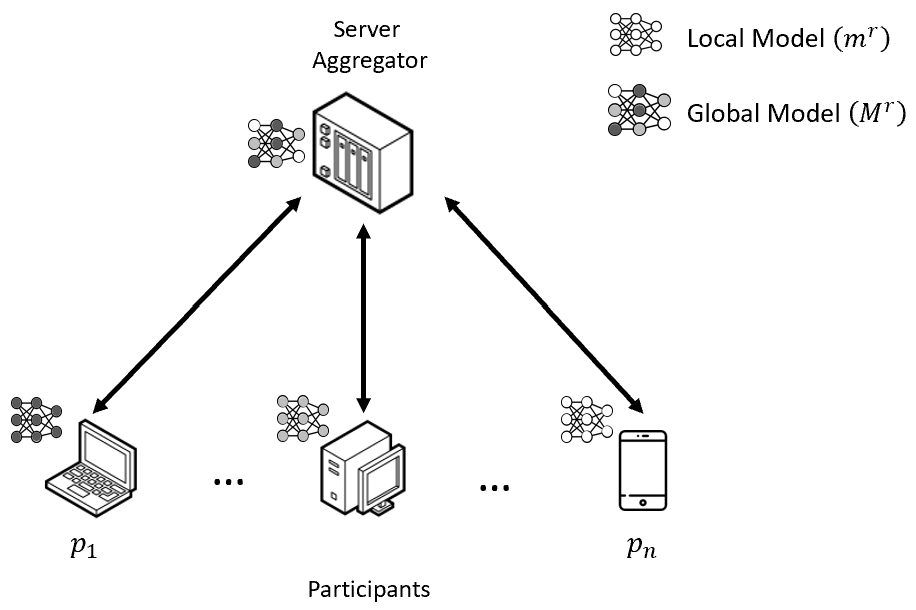
\includegraphics[width=0.85\textwidth]{/Users/mukeshch/Downloads/arXiv-2502.14464v1/Images/1.png}
  \caption{Registration and initial key publication (source paper figure).}
  \label{fig:registration}
\end{figure}

\subsection*{Session establishment}
After registration, the server and a participant exchange messages off-chain to establish shared secrets. The server sends its KEM public key and ECDH public key (signed using the server's blockchain private key) off-chain to the participant. The participant validates the signature using the server's blockchain public key and then performs Kyber encapsulation to obtain a KEM ciphertext and shared secret, and computes an ECDH shared secret. The concatenation of the KEM shared secret and the ECDH shared secret is input into the asymmetric KDF to derive the root key $\mathrm{RK}$. The analogous steps performed by the participant (sending its ECDH public key and the KEM ciphertext) allow the server to compute the same root key. The sequence is shown in Figure~\ref{fig:session}.

\begin{figure}[H]
  \centering
  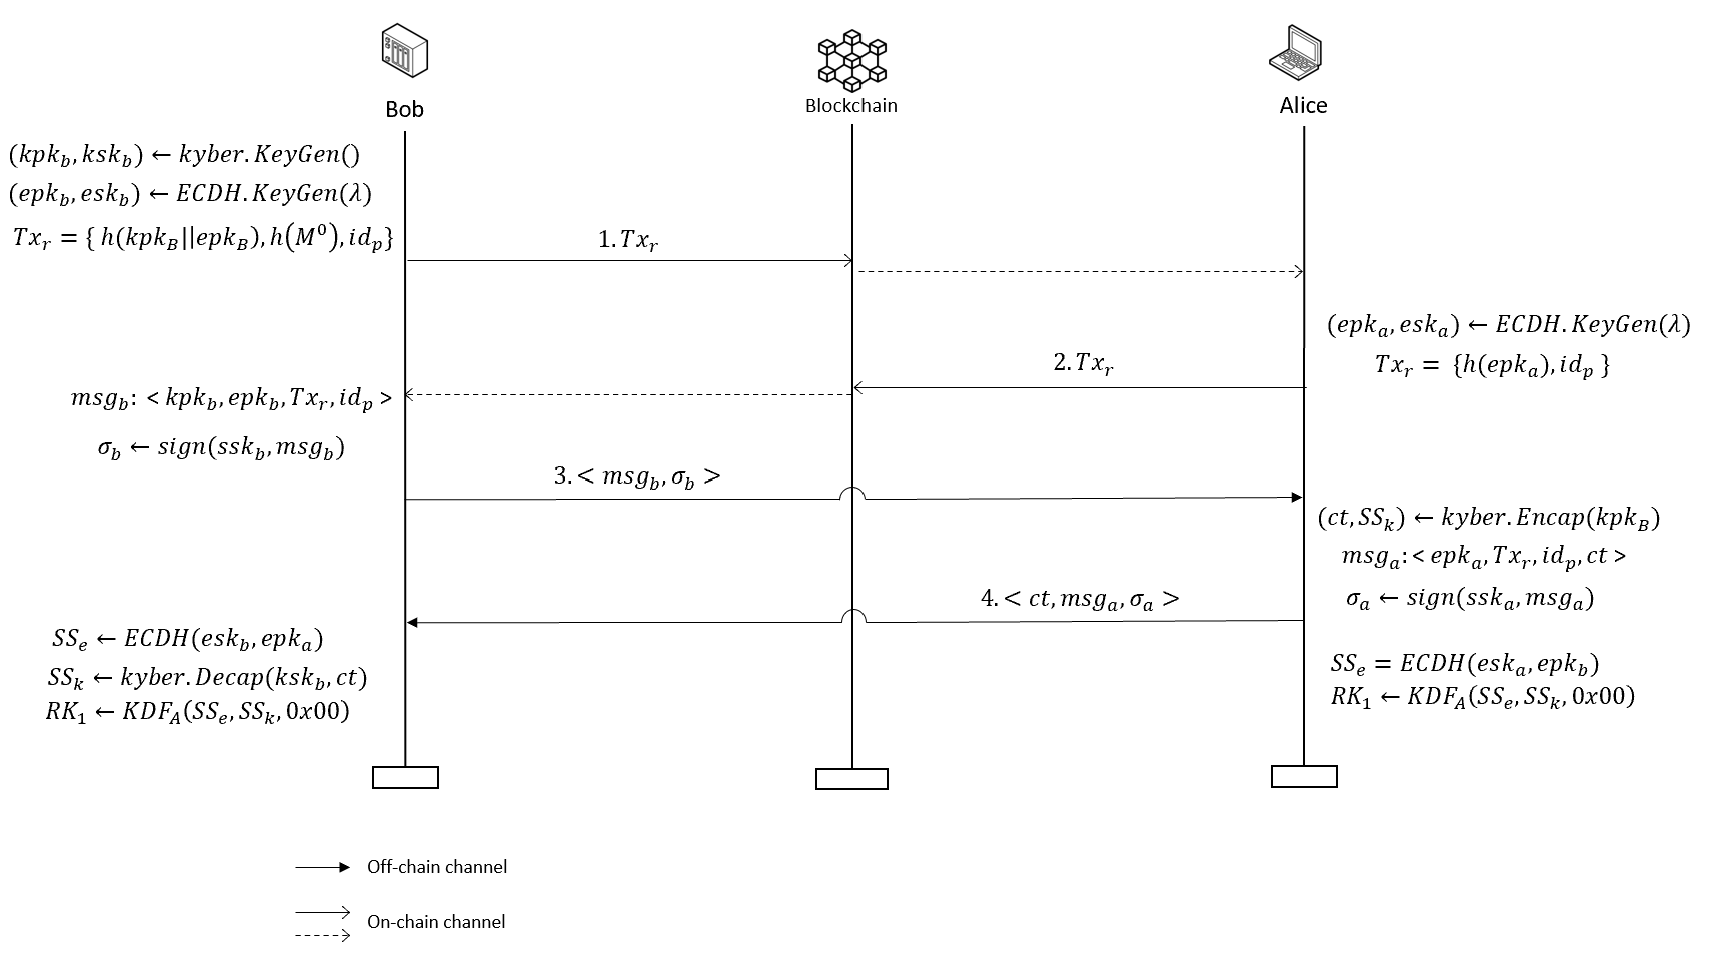
\includegraphics[width=0.9\textwidth]{/Users/mukeshch/Downloads/arXiv-2502.14464v1/Images/3.png}
  \caption{Session establishment and key derivation (KEM + ECDH $\rightarrow$ root key).}
  \label{fig:session}
\end{figure}

\subsection*{Publish task and model transfer (per round)}
For each training round $r$, the server publishes a Task transaction containing the round number, project/task IDs, and the hash of the wrapped global model information. Using the previously derived root key, the server derives chain keys and per-round model keys using the symmetric KDF. The server encrypts per-round payloads with the derived model key and sends signed encrypted messages off-chain to participants; it also publishes minimal metadata (hashes and deadlines) on-chain. Participants decrypt the off-chain payload using the same model key, perform local training, and then send an Update transaction (containing the hash of the participant's encrypted model information) on-chain while sending the encrypted model off-chain. The server then authenticates, decrypts, evaluates the model, aggregates accepted updates, and publishes Feedback transactions with scores. Figure~\ref{fig:send_receive} illustrates the send/receive flow for a single training round.

\begin{figure}[H]
  \centering
  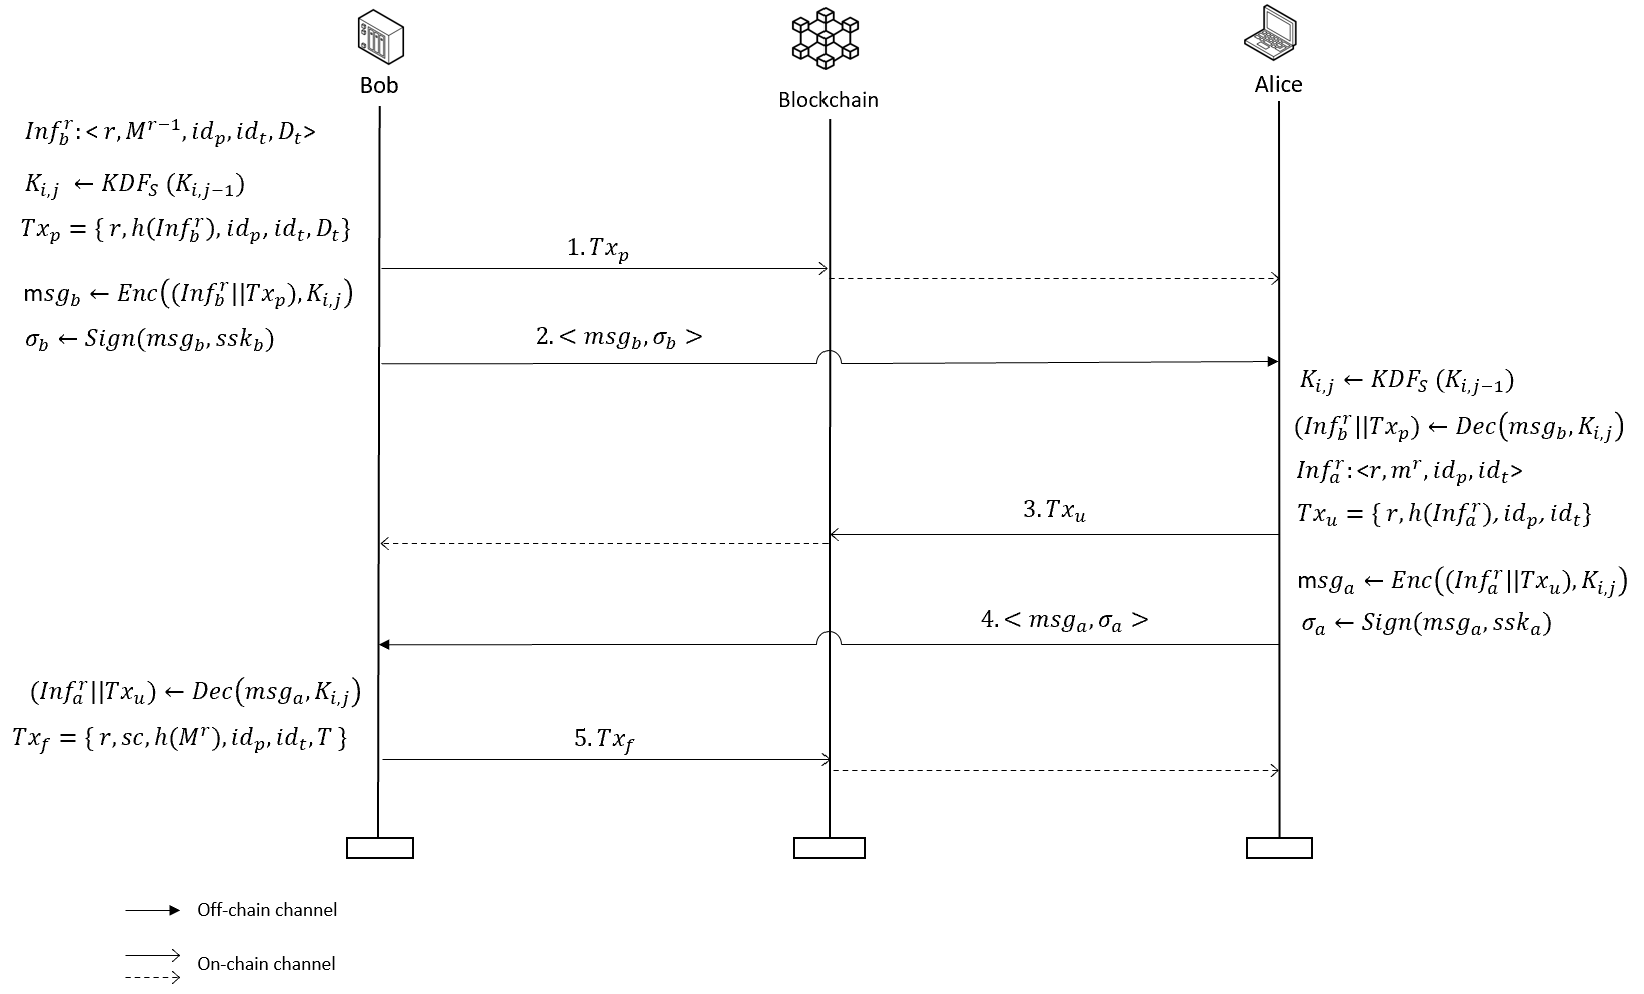
\includegraphics[width=0.95\textwidth]{/Users/mukeshch/Downloads/arXiv-2502.14464v1/Images/4.png}
  \caption{Send and receive model flow for a single training round (publish, update, feedback).}
  \label{fig:send_receive}
\end{figure}

\subsection*{Ratchet mechanism (forward secrecy and post-compromise security)}
PQBFL combines symmetric and asymmetric ratcheting:
\begin{itemize}
  \item \textbf{Symmetric ratchet:} From the root key $\mathrm{RK}_j$, the participants and server derive a chain key $\mathrm{CK}_{i,j}$ and then a model key $\mathrm{K}_{i,j}$ for each symmetric step $i$ within asymmetric ratchet period $j$ using the symmetric KDF. After using a model key for encryption/decryption in round $r$, the key is discarded to ensure forward secrecy for earlier rounds.
  \item \textbf{Asymmetric ratchet:} After a server-determined threshold of symmetric steps ($L_j$), the server triggers an asymmetric ratchet by generating new KEM and ECDH key pairs and publishing their hashes in the next Publish Task transaction. Participants receive the new public keys, perform encapsulation/EC Diffie-Hellman calculations to derive new shared secrets, and input them into the asymmetric KDF to obtain a fresh root key $\mathrm{RK}_{j+1}$, restoring post-compromise security.
\end{itemize}

Figure~\ref{fig:ratchet} gives a condensed illustration of alternating asymmetric and symmetric ratchets and how model keys are derived for consecutive rounds.

\begin{figure}[H]
  \centering
  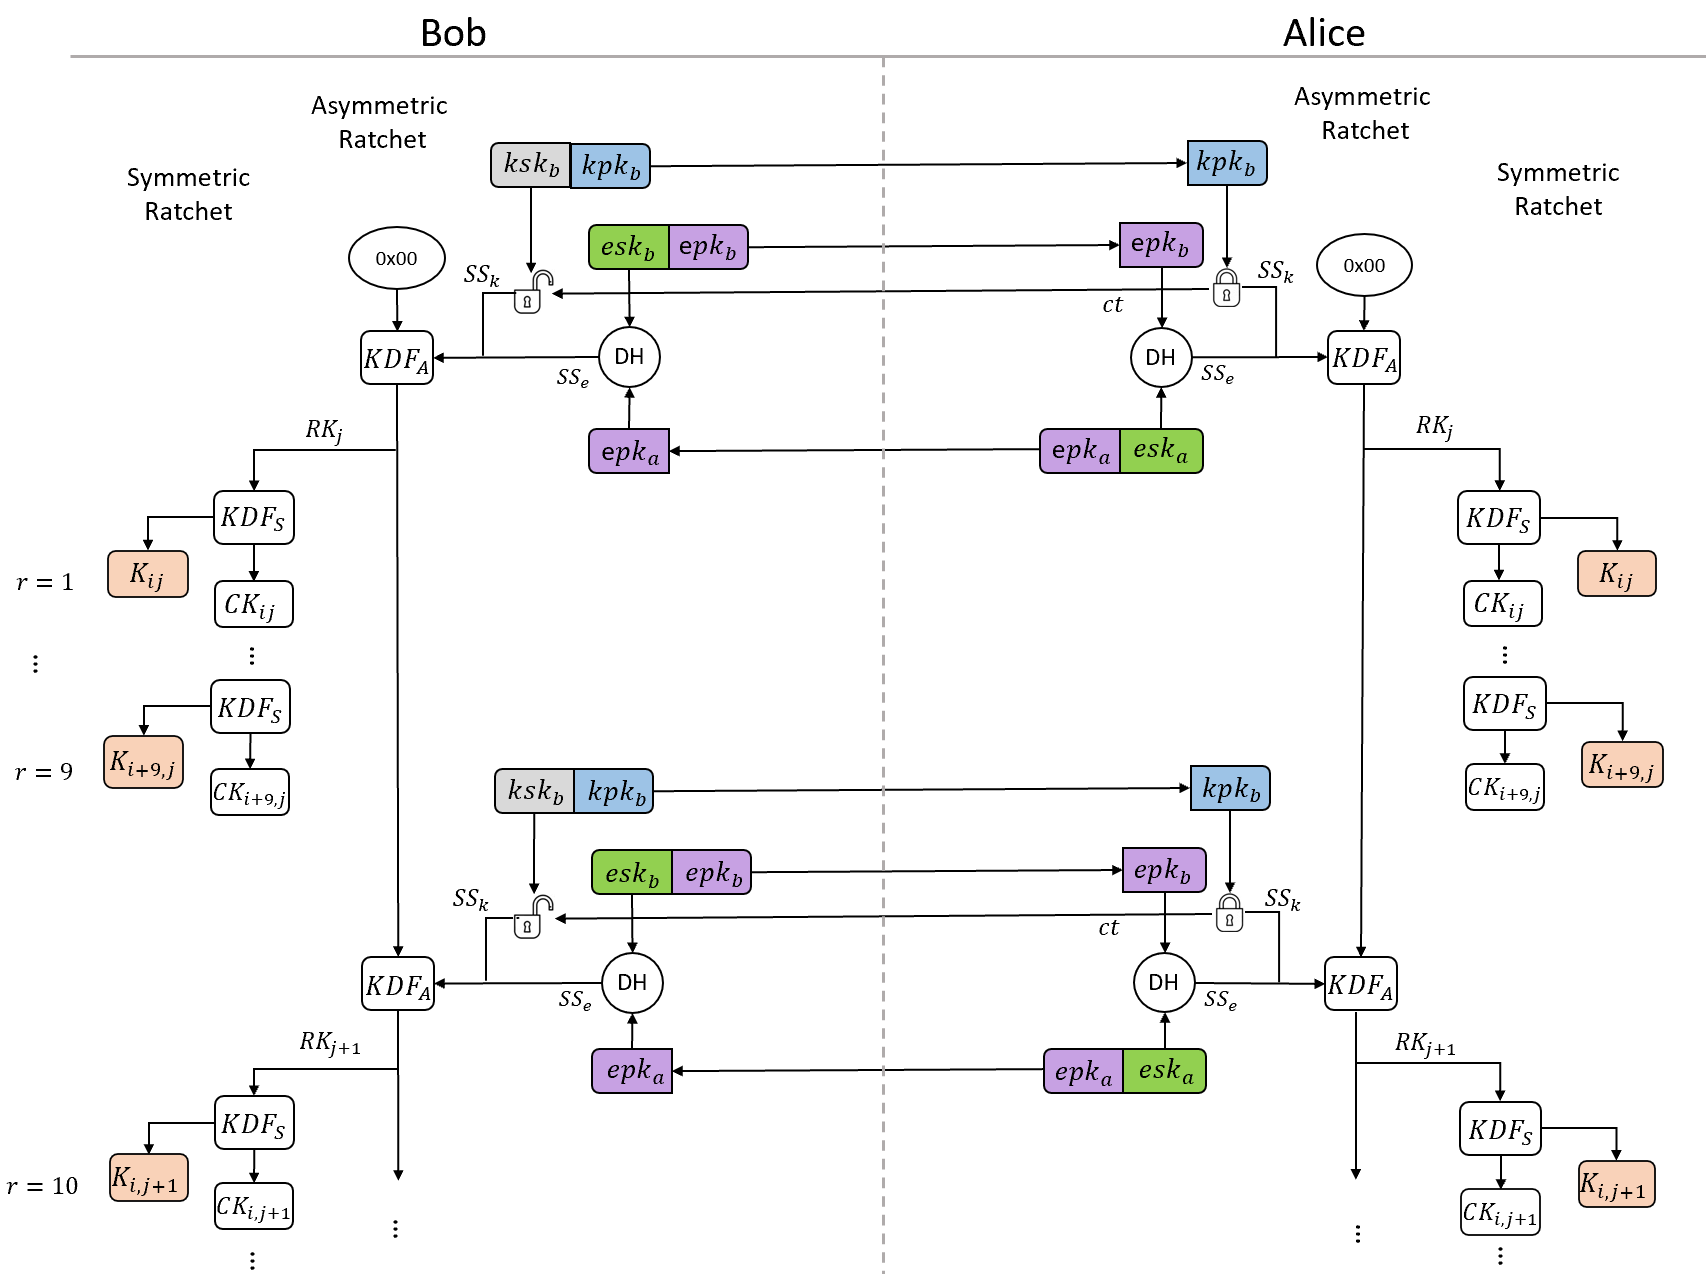
\includegraphics[width=0.95\textwidth]{/Users/mukeshch/Downloads/arXiv-2502.14464v1/Images/5.png}
  \caption{Overview of symmetric and asymmetric ratcheting across multiple rounds.}
  \label{fig:ratchet}
\end{figure}

\subsection*{Security considerations and mitigations}
The combined use of Kyber (KEM) and ECDH in a hybrid construction reduces the risk of single-point cryptographic failure (the protocol remains secure if at least one primitive remains unbroken). Ratcheting enforces forward secrecy and (when the asymmetric ratchet occurs) post-compromise security. Blockchain provides tamper-evident recording of registration, task publication, and update hashes which supports accountability and reputation management while keeping bulk model transfers off-chain reduces gas and storage costs.

\subsection*{Figures referenced from the arXiv bundle}
The images used in this file are taken from the downloaded arXiv bundle at:
\begin{verbatim}
/Users/mukeshch/Downloads/arXiv-2502.14464v1/Images/
\end{verbatim}
If you move images into the project workspace (recommended), update the included paths to relative locations (for example, `Images/3.png`).

\section*{Acknowledgements}
This methodology section references the PQBFL paper by Gharavi et al. (2025). All figures used are reproduced from the paper's figure bundle attached by the user.

\end{document}
